\documentclass[fontsize=10pt,openright,oneside,paper=a4,BCOR=1cm,numbers=noenddot]{scrbook}


\usepackage[top=3.5cm, bottom=3.5cm, left=3.0cm, right=4.0cm]{geometry}
\usepackage{lipsum}
\usepackage{tabularx}
\usepackage{hyperref}


%%%%%%%%%%%%%%%%%%%%%%%%%%%%%%%%%%%%%%%%%%%%%%%%%%%%%%%%%%%%
% Basic definitions, to be adjusted individually
\newcommand{\authornamefirstone}{Tim}
\newcommand{\authornamelastone}{Greller}
\newcommand{\matrikelnummerone}{102871}
\newcommand{\authornamefirsttwo}{Jonas}
\newcommand{\authornamelasttwo}{Heitz}
\newcommand{\matrikelnummertwo}{102939}
\newcommand{\authornamefirstthree}{Sebastian}
\newcommand{\authornamelastthree}{Pretzsch}
\newcommand{\matrikelnummerthree}{103114}
\newcommand{\authornamefirstfour}{Finn}
\newcommand{\authornamelastfour}{Ribbeck}
\newcommand{\matrikelnummerfour}{102876}
\newcommand{\authornamefirstfive}{Emily}
\newcommand{\authornamelastfive}{Vorderwülbeke}
\newcommand{\matrikelnummerfive}{103087}
\newcommand{\authors}{{\authornamefirstone~\authornamelastone, \authornamefirsttwo~\authornamelasttwo,
            \authornamefirstthree~\authornamelastthree, \authornamefirstfour~\authornamelastfour,
            \authornamefirstfive~\authornamelastfive}}

\newcommand{\worktitle}{DDos Attacks inside a Simulation Suite for Network Slicing in 5G Networks}

\newcommand{\thesistype}{Advanced Security Engineering Lab}
\newcommand{\courseofstudies}{Summer Term 2022}

\newcommand{\thesisdate}{2022--09--21}   %% in ISO 8601 format

\newcommand{\thesisprof}{Dr.-Ing. Tolga Arul}
\newcommand{\chair}{\mbox{Chair of Computer Engineering}}

\newcommand{\advisor}{Felix Klement}


\newcommand{\contactprofone}{
\thesisprof \\
\chair \\
Universität Passau \\
Email:~{\small \url{tolga.arul@uni-passau.de}}  \\
Web:~{\small
\url{https://www.fim.uni-passau.de/en/computer-engineering/}}\\}

%\newcommand{\drosera}{\textit{Drosera}\xspace}
%%%%%%%%%%%%%%%%%%%%%%%%%%%%%%%%%%%%%%%%%%%%%%%%%%%%%%%%%%%%

% PACKAGES:

\usepackage{color}
\usepackage[colorinlistoftodos,prependcaption]{todonotes}
\usepackage{xargs}

\newcommandx{\mytodo}[2][1=]{\todo[linecolor=yellow,backgroundcolor=yellow!25,bordercolor=yellow,inline,#1]{#2}}

% Use English :

% Use list of tabels, etc. in table of contents:
\usepackage[nottoc]{tocbibind}
% German paragraph skip
\usepackage{parskip}
% Encoding. Use utf8. We are now in the 21st century already... :-)
\usepackage[utf8]{inputenc}
% Index-generation
\usepackage{makeidx}
% Einbinden von URLs:
\usepackage{url}
% Special \LaTex symbols (e.g. \BibTeX):
\usepackage{doc}
% Include Graphic-files:
%\usepackage{graphics}
% Include Graphic-files:
\usepackage{graphicx}
% Include doc++ generated tex-files:
%\usepackage{docxx}
% Include PDF links
\usepackage{listings}
\usepackage{float}
\usepackage{pgfplots}
\usepackage{multirow}
%mathstuff
\usepackage[cmex10]{amsmath}
\usepackage{amsfonts}
\usepackage{amssymb}
\usepackage{longtable}
\usepackage{pgf-pie}
\usepackage{pifont}% http://ctan.org/pkg/pifont
\newcommand{\cmark}{\ding{51}}%
\newcommand{\xmark}{\ding{55}}%
\usepackage{pdfpages}
\usepackage{multicol}
\usepackage{xspace}
\newcounter{mtpage}

% TODOOOOO
%hyperref for nice PDF output
%\usepackage[pdftex, 
%bookmarks=true,
%pdfauthor={authors},
%pdftitle={{{\worktitle}}},
%hidelinks
%]{hyperref}

%%%%%%%%%%%%%%%%%%%%%%%%%%%%%%%%%%%%%%%%%%%%%%%%%%%%%%%%%%%%

% OTHER SETTINGS:

\pgfplotsset{compat=1.18}

% Pagestyle:
\pagestyle{headings}

% Avoid 'overhang':
\sloppy

% Choose language
\newcommand{\setlang}[1]{\selectlanguage{#1}\nonfrenchspacing}

\usepackage[english]{babel}

\setlang{english}
%\setlang{german}

\usepackage[Bjornstrup]{fncychap}

\definecolor{bblue}{HTML}{00A2FF}
\definecolor{rred}{HTML}{FF2600}
\definecolor{ggreen}{HTML}{61D836}
\definecolor{ppurple}{HTML}{C24885}
\definecolor{oorange}{HTML}{F8BA00}
\definecolor{ggray}{HTML}{5F5F5F}
\definecolor{ppink}{HTML}{e81cbf}


%%%%%%%%%%%%%%%%%%%%%%%%%%%%%%%%%%%%%%%%%%%%%%%%%%%%%%%%%%%%

% TITLE:

\begin{document}
\frontmatter
\thispagestyle{empty}
\newpage

\vspace{1cm}

\begin{center}
\begin{tabular}{lr}

\includegraphics[width=6.5cm]{img/logouni_en.png}
\end{tabular}

\vspace{3cm}
\Large University of Passau
\\
\Large Faculty of Computer Science and Mathematics
\\
\vspace{0.3cm}
\Large {\chair }
\\
\Large \thesisprof

\end{center}


\vspace{2.5cm}

\begin{center}
        % Master's thesis, Bachelor's thesis, Programming project
        {\Large \thesistype 
        
        \courseofstudies} 
\end{center}

\begin{center}
        \settowidth{\baselineskip}{0.4cm}
        {\LARGE \textbf{\worktitle}}
        \\
        {\Large
        \vspace{1cm}
        \authornamefirstone~\authornamelastone~\textit{\matrikelnummerone} \\
        \authornamefirsttwo~\authornamelasttwo~\textit{\matrikelnummertwo} \\
        \authornamefirstthree~\authornamelastthree~\textit{\matrikelnummerthree} \\
        \authornamefirstfour~\authornamelastfour~\textit{\matrikelnummerfour} \\
        \authornamefirstfive~\authornamelastfive~\textit{\matrikelnummerfive} \\
        }
\end{center}

\vfill {% \settowidth{\baselineskip}{0.2cm}

\vfill


{\large
\begin{tabular}[l]{llll}

Date:       & \thesisdate %%(\LaTeX{}$2_\epsilon$ run \today)
\smallskip \\
Supervisor:   & \thesisprof \\
Advisor: & \advisor \\
\end{tabular}}
} \cleardoublepage
%%%%%%%%%%%%%%%%%%%%%%%%%%%%%%%%%%%%%%%%%%%%%%%%%%%%%%%%%%%%

% MAIN PART:

% Abstract. 
%!TEX root = ../thesis.tex

\thispagestyle{plain}

\section*{Abstract}

As 5G is a relatively new technology that is gaining relevance, the threat of \textit{distributed denial-of-service} (DDoS) is an important problem.

To explore the effects of DDoS attacks, this project shows an implementation and validation of DDoS attacks in a simulated 5G network, using the simulation framework ns-3 with 5G-Lena. Further the implications and benefits network slicing has in this context are demonstrated. 
Using the tracing system provided by ns-3, a custom tracing implementation and NetAnim, data was gathered that show the dropping bandwidth during DDoS attacks and the successful separation of the slices, so that only the slices where attacks are present suffer from its effects.

The chosen implementation style though could not be used to dynamically isolate the attacker on a slice. Conclusions were drawn to help guide future implementations.

% Table of contents
\tableofcontents

% Main body of thesis
\mainmatter
% !TeX encoding = UTF-8
% !TeX spellcheck = en_GB
% !TeX root = ../thesis.tex


\chapter{Introduction}
\label{chapter:introduction}

5G Networks have a growing relevance worldwide due to its improvements in speed, capacity and latency. A report stated 94 percent of respondents expect 5G growth to increase security and reliability concerns among 5G mobile operators, literature suggests that the potential threat of DDoS attacks has increased and is among the most serious attacks of all in 5G networks, since it prevents users from accessing network services \cite{huang2021trend}. Network slicing is one od the main features, that will bring 5G to the next level \cite{zhang2019overview}. But especially the performance and availability of network slices can be impacted by these types of attacks because they can share physical resources among each other. Therefore the interest in finding methods to manage these attacks is on the rise. A useful tool against this approach can be slice isolation, which is also an essential requirement for 5G networks \cite{sattar2019towards}.

To get a better understanding of the procedure of DDoS attacks and of potential measures against them, we want to focus on the following research questions:
\begin{addmargin}[20pt]{0pt}
    \begin{itemize}
        \item \textbf{RQ1: }\textit{What are the effects of DDoS attacks in a 5G network?}
        \item \textbf{RQ2: }\textit{What benefits does slicing have in case of DDoS attacks?}
    \end{itemize}
\end{addmargin}

For Background this paper will go over 5G networks in general, network slicing and the upcoming relevance of DDos attacks in 5G networks. The main focus will be on the implementation of the simulation using ns-3 with 5G-Lena and the data gathering process. Lastly the collected data will be visualized, evaluated and discussed.
% !TeX encoding = UTF-8
% !TeX spellcheck = en_GB
% !TeX root = ../thesis.tex

\chapter{Background}
\label{chapter:background}
\section{5G Network}
5G networks are cellular networks, in which the service area is divided into small geographical areas called cells. All 5G wireless devices in a cell communicate by radio waves with a cellular base station via fixed antennas, over frequency channels assigned by the base station. The base stations, termed nodes, are connected to switching centers in the telephone network and routers for Internet access by high-bandwidth optical fiber or wireless backhaul connections. As in other cellular networks, a mobile device moving from one cell to another is automatically handed off seamlessly.


The 5G system architecture is defined in TS 23.501. The most relevant parts of the system architecture are the Radio Access Network (RAN), which in 5G Networks is called 5G New Radio (5G NR), and the Core Network. The packet protocol for mobility management (establishing connection and moving between base stations) and session management (connecting to networks and network slices) is described in TS 24.501. Specifications of key data structures are found in TS 23.003.


Frequency bands for 5G NR, which is the air interface or radio access technology of the 5G mobile networks, are separated into two different frequency ranges, this is defined in TS 38.101. First there is Frequency Range 1 (FR1), which includes sub-6 GHz frequency bands, some of which are traditionally used by previous standards, but has been extended to cover potential new spectrum offerings from 410 MHz to 7125 MHz. The other is Frequency Range 2 (FR2), which includes frequency bands from 24.25 GHz to 71.0 GHz. These frequency ranges are used on different bands depending on in which country the 5G network is located in \cite{zhang2017overview}. 

\section{Slicing}
Network slicing separates the network into multiple logical networks. Each logical network is designed to serve a defined business purpose and comprises of all the required network resources, configured and connected end-to-end. 
The underlying purpose of network slicing is to guarantee different users different Qualities of Service (QoS).
Since the range of use case scenarios of the 5G network is very diverse one can not guarantee every QoS for every user, hence the need for slicing.

Standards exist, but the implementation of network slicing depends on the service provider. Due to this there is not much to be found on how to implement slicing. 
The standards are regulated by the 3rd Generation Partnership Project (3GPP). The most important standards for slicing are the TS 22.261 (Version 18.6.1) and TS 23.501 (Version 17.5.0).

In TS 23.501 the 3GPP defined five different Slice/Service Types (SST):
\begin{table}
\begin{tabularx}{\textwidth}{c|c|p{8cm}}
\textbf{Slice/Service Types} & \textbf{SST value} & \textbf{Characteristics} \\
\hline
  eMBB   & 1 & Slice suitable for the handling of 5G enhanced Mobile Broadband. \\
  URLLC   & 2 & Slice suitable for the handling of ultra- reliable low latency communications. \\
  MIoT   & 3 & Slice suitable for the handling of massive IoT. \\
  V2X   & 4 & Slice suitable for the handling of V2X services. \\
  HMTC   & 5 & Slice suitable for the handling of High-Performance Machine-Type
Communications. \\
\end{tabularx}
\caption{Slice/Service Types}
\label{t:slice/service types}
\end{table}

% TODO: Tomaso?
In most implementations frequencies are dynamically assigned in order to guarantee the corresponding values for the SST. The values that are relevant include the data rate, latency and low packet loss.

\section{DDoS Attack in 5G Networks}
\subsection{DDos Attack}
Denial-of-service attack (DoS attack) is a cyber-attack in which the perpetrator seeks to make a machine or network resource unavailable to its intended users by temporarily or indefinitely disrupting services of a host connected to a network. Denial of service is typically accomplished by flooding the targeted machine or resource with superfluous requests in an attempt to overload systems and prevent some or all legitimate requests from being fulfilled.

In a distributed denial-of-service attack (DDoS attack), the incoming traffic flooding the victim originates from many different sources. More sophisticated strategies are required to mitigate against this type of attack, as simply attempting to block a single source is insufficient because there are multiple sources.

\subsection{Relevance of DDoS Attacks in 5G Networks}
Due to the improved capabilities of 5G Networks in regards to speed, capacity and latency the threat of DDoS Attacks has increased since malicious parties can also use these improved capabilities. Here network slicing can potentially help on isolating malicious parties onto a separate slice, where they can not harm anyone.\cite{sattar2019towards}

% !TeX encoding = UTF-8
% !TeX spellcheck = en_GB
% !TeX root = ../thesis.tex

\chapter{Implementation}
\label{chapter:implementation}
\section{General Setup}

The following setup guide describes how ns-3, 5G-Lena can be setup fresh in a development environment for your own use. If you would like to use the simulation that we implemented for this project, you can skip to the installation guide at~\ref{section:install-project}.

\subsection{ns-3 Setup}

The following is a setup guide to install and build\footnote[1]{\url{https://www.nsnam.org/docs/tutorial/html/getting-started.html}} ns-3 on Mac OS and Linux. Unfortunately it doesn't run on Windows natively and you need a WSL/VM. 

\subsubsection{Prerequisites}
\begin{itemize}
    \item C++ compiler: clang++ or g++
    \item Python: python3 version $\geq$ 3.6
    \item cmake version $\geq$ 3.10
    \item Build system: make, ninja, (xcodebuild necessary for Mac OS)
\end{itemize}

\subsubsection{Installation}

In order to use git to save your own commits fork the official ns-3 GitLab Repository\footnote[2]{\url{https://gitlab.com/nsnam/ns-3-dev}}. After you successfully forked the repository clone it onto your computer. Next open a terminal window in the repository folder. You then have to checkout the desired version of ns-3 by checking out the corresponding tag. (It's recommended to create a branch starting at this tag.) 

\subsubsection{Building ns-3}

\begin{enumerate}
    \item In order to configure ns-3 enter: \begin{verbatim}
    ./ns3 configure --enable-examples --enable-tests
\end{verbatim}
\item To build ns-3 enter: \begin{verbatim}
    ./ns3
\end{verbatim}
    You will see a lot of compiler output messages. This command also runs the enabled tests. Here it is important that all the tests pass and none fail or crash.
\end{enumerate}

\subsubsection{Running scripts via the command line}

Run your first file by entering: 
\begin{verbatim}
    ./ns3 run hello-simulator
\end{verbatim}
Your output should be: \textit{Hello Simulator}.

\subsection{Running your own scripts}

Create a new \textit{.cc} file in the \textit{scratch} folder, or copy an existing example into the scratch folder. For the compiler to recognize your script in the \textit{scratch} folder you must add: \begin{verbatim}
    \ingroup scratch
    \file {filename}
\end{verbatim} in a doxygen comment right at the beginning of the file. You can now run your script.

\subsection{5G-Lena simulator}
In order to use the 5G-Lena module\footnote[5]{\url{https://5g-lena.cttc.es/}} to simulate a 5G network you unfortunately had to write the 5G-Lena project an email to request access to their GitLab-Repository.

\textit{Update:} The GitLab-Repository to access the 5G-Lena module, that simulates a 5G network, is now openly accessible\footnote[6]{\url{https://gitlab.com/cttc-lena/nr}}.
To use the module either clone the repository or add it as a submodule into \textit{./contrib}.

\section{Download, Install and Run the simulation of this project}
\label{section:install-project}

\subsection{Clone this repository with the ns-3 and LENA submodules}
You can use Git on the command-line to clone our repository that holds all submodules using the following command:

\begin{verbatim}
git clone --recurse-submodules git@git.fim.uni-passau.de:klement/ase-lab-ss22-ddos-simulation.git
\end{verbatim}

This requires you to have:
\begin{enumerate}
    \item SSH keys setup for the FIM GitLab, gitlab.com and github.com
    \item Access to our custom ns-3-dev fork\footnote[7]{\url{https://gitlab.com/DerBambus/ns-3-dev}}.
    \item Access to our custom LENA nr fork\footnote[8]{\url{https://gitlab.fim.uni-passau.de/greller/nr}}.
\end{enumerate}

If you already cloned this repository without \texttt{--recurse-submodules}, then run:
\begin{verbatim}
git submodule update --init --recursive --remote
\end{verbatim}

\subsection{Build ns-3}
From here on we assume you are using a Debian based Linux.

Next the minimal required packages are installed:
\begin{verbatim}
apt install libsqlite3-dev g++ python3 python3-dev pkg-config sqlite3 cmake
\end{verbatim}
Optionally the qt5 packages required for the NetAnim animator can be installed now if you want to use NetAnim.
\begin{verbatim}
apt install qtbase5-dev qtchooser qt5-qmake qtbase5-dev-tools
\end{verbatim}
With everything installed, you can configure and build ns-3 as follows:
\begin{verbatim}
./ns3 configure --enable-examples
./ns3
\end{verbatim}
If the ns-3 configure shows missing dependencies, these have to be installed prior to starting the build.  
To confirm that the build was successful you can try out the examples, e.g.:
\begin{verbatim}
./ns3 run simple-global-routing
\end{verbatim}
This creates \texttt{simple-global-routing.*} output files. You can take a look at the text trace file like this:
\begin{verbatim}
cat simple-global-routing.tr
\end{verbatim}

\subsection{Install NetAnim}
NetAnim uses the mercurial version control system. In order to download NetAnim, you first need to install the necessary mercurial prerequisite.
\begin{verbatim}
apt install mercurial
\end{verbatim}
Clone the NetAnim repository's files using mercurial and enter the new directory:
\begin{verbatim}
hg clone http://code.nsnam.org/netanim
cd netanim
\end{verbatim}
Now you can build NetAnim using Makefiles.
\begin{verbatim}
qmake NetAnim.pro
make
\end{verbatim}
This produced a NetAnim executable which can be started as follows.
\begin{verbatim}
./NetAnim
\end{verbatim}
NetAnim can be used to load and visualize the XML-files produced during simulation.  
You can test NetAnim with the XML-files generated by the examples in \texttt{src/netanim/examples}:
\begin{verbatim}
./ns3 run "dumbbell-animation --nLeftLeaf=5 --nRightLeaf=5 --animFile=dumbbell.xml"
./ns3 run "star-animation --animFile=star.xml"
\end{verbatim}

\subsection{Execute the Projects Simulation}
If you have configured ns-3 successfully, you can run our Lab-Demo script file using the following command:
\begin{verbatim}
./ns3 run lab-demo
\end{verbatim}
This uses the default settings where DoS attacks are disabled and the first scenario is used. To run our simulation with custom values, you can specify several parameters:
\begin{verbatim}
./ns3 run lab-demo -- --dosMMTC=true --botAmount=5 --scenario=2
\end{verbatim}
In the above example DDoS is executed on the MMTC slice only using 5 bots per base station and the second scenario is used.

\section{IDE Setup}

In order to run ns-3 from VS Code install the following extensions:\footnote[3]{\url{https://www.youtube.com/watch?v=Ab8eYHhT5I8}}
\begin{itemize}
    \item C/C++ (When using Arch Linux either use Clangd Highlighting or install C/C++ manually.\footnote[4]{\url{https://marketplace.visualstudio.com/items?itemName=ms-vscode.cpptools}})
    \item CMake
    \item CMake Tools
\end{itemize}
You now can run your ns-3 scripts via the CMake extension.

\textbf{If your build is continuously not successful turn off} \begin{verbatim}
    NS3_WARNINGS_AS_ERRORS
\end{verbatim} \textbf{in the root CMakeLists.txt.}

\section{Implementation details}
    Our base simulation is based on standard 5G-Lena examples. Therefore we will not go too in depth on explaining that part of the simulation.
    Mainly we will focus on our take on slicing.
    
    \subsection{Network slicing}
    In most slicing implementations frequencies are dynamically assigned to the slices. However this frequency allocation relies heavily on environmental variables such as the terrain. Therefore we decided to assign frequencies statically based on their capabilities to help guarantee QoS, data rate and latency, e.g.: high frequency for high data rate.
    
    In our slicing implementation the slicing guarantees are made by two factors, the aforementioned static frequency allocation and 5G-Lena's core network calculations which in turn are specified by the EPSBearer. 
    
    The EPSBearer serves as a functional component of the frequency band. By allocating this EPSBearer to a band 5G-Lena is instructed to ensure these QoS guarantees.
    
    \subsection{Technical details}
    In 5G-NR there are five slicing types as mentioned in Table \ref{t:slice/service types}. We only focused on the following three:
    \begin{itemize}
        \item eMBB: Enhanced mobile broadband
        \begin{itemize}
            \item Used for high mobility in macro and small cells and for a reduced power consumption.
            \item SST value: 1
            \item Frequency: 28 GHz
            \item Bandwidth: 4000 MHz
            \item Subcarrier spacing: 15 KHz
            \item Data rate: 20 Gbp/s
            \item EPSBearer: \verb!NGBR_LOW_LAT_EMBB!
        \end{itemize}
        \item mMTC: massive machine type communication
        \begin{itemize}
            \item Used for long range connectivity with a low data rate and low cost for machine to machine communication.
            \item SST value: 5
            \item Frequency: 700 MHz
            \item Bandwidth: 5 MHz
            \item Subcarrier spacing: 30 KHz
            \item Data rate: 1-100 Kbp/s
            \item EPSBearer: \verb!DGBR_ITS! 
        \end{itemize}
        \item URLLC: Ultra reliable low latency communication
        \begin{itemize}
            \item Used for ultra responsive connections between multiple devices.
            \item SST value: 2
            \item Frequency: 3.5 GHz
            \item Bandwidth: 100 MHz
            \item Subcarrier spacing: 60 KHz
            \item Data rate: 50 Kbp/s - 10 Mbp/s
            \item EPSBearer: \verb!DGBR_DISCRETE_AUT_SMALL!
        \end{itemize}
    \end{itemize}
    
    \subsection{Scenarios}
    There are four different scenarios with different amounts of base stations and user entities that can be selected.
    - 1. Scenario:
	    - 1 GnB
	    - 5 UE per GnB -> Distributed on the three slices.
    - 2. Scenario:
	    - 2 GnB
	    - 10 UE per GnB -> Distributed on the three slices.
    - 3. Scenario:
	    - 2 GnB
	    - 10 stationary UE per GnB ->  Distributed on the three slices.
	    - 10 mobile UE per GnB -> Distributed on the three slices.
        - TODO: Mobility has yet to be implemented.
    - 4. Scenario:
	    - 5 GnB
	    - 40 UE per GnB -> Distributed on the three slices.
        - TODO: Allocate slice type, mobile/stationary random.
    
    \subsection{DDoS simulation}
    Our DDoS simulation is capable of attacking each aforementioned slicing type. To do so you have to give the desired slice type (``dosURLLC'', ``dosMMTC'', ``dosEMBB'') and the amount of bots that are flooding the server in the DoS-Attack (``botAmount'') as a command line argument. If turned on the slice type flag enables the part of the code, where the bots are activated. 
    The bots are a simple ns3-OnOffApplication with the corresponding EPSBearer that runs on the specified slice.
    The bots use a separate remote host with a UDP packet sink.    
% !TeX encoding = UTF-8
% !TeX spellcheck = en_GB
% !TeX root = ../thesis.tex

\chapter{Tracing and Visualization}
\label{chapter:tracing}

\section{Basic Metrics of the Packet Flows}
\section{Trace data of all Device Operations with Packets}
\section{Tracing and 5G New Radio}

% !TeX encoding = UTF-8
% !TeX spellcheck = en_GB
% !TeX root = ../thesis.tex

\chapter{Evaluation and Discussion}
\label{chapter:evaluation}
\section{Learning from the data}
    The most important finding is, that slice isolation works. That means if one slice is under a DDos attack, other slices will be unaffected. This can be seen in the following graphs:
    
    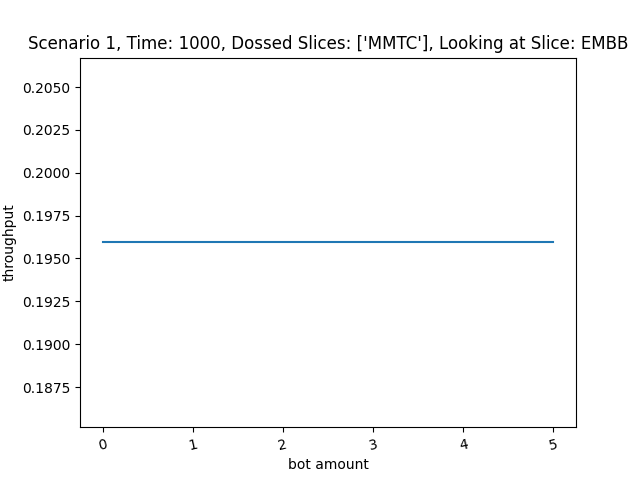
\includegraphics[width=\textwidth]{img/slice_isolation_works_single.png}
    
    This first graph shows, that the DDos attack on a slice (MMTC) has no effect on a different slice (EMBB).
    
    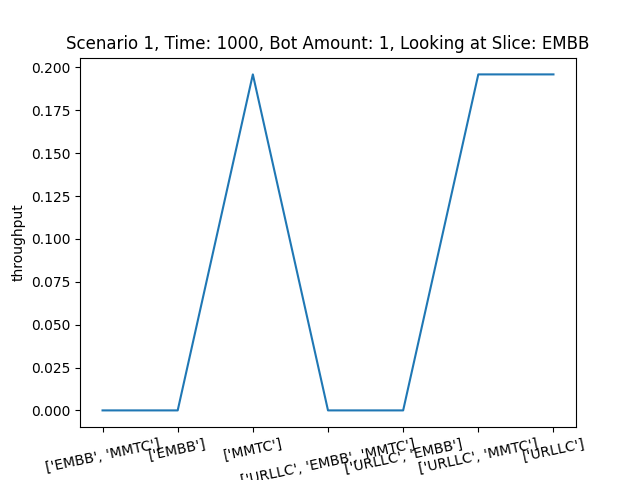
\includegraphics[width=\textwidth]{img/slice_isolation_works_dossed_slices.png}
    
    This second one shows the same point across all possible slice attacks. Only when the EMBB slice is under the attack the throughput of it decreases. This answers our second research question, that slice isolation is a useful tool as a counter measure against DDos attacks.\\
    Data evaluation can also be used in later stages from other teams. Inside our Jupyter Notebook are tools to continue the data evaluation.
    
\section{Problems with the Implementation}
    \subsection{Slicing and Machine Learning}
    Our analysis has shown that slicing prevents attacker nodes from influencing the traffic happening on other slices where no DoS-nodes are present. This enables us to isolate nodes that are executing the DDoS attack on their own slice. This way they would only influence each other.
    
    But due to our slicing implementation relying heavily on computational efforts provided by the 5G Lena network in addition to mainly using the EPSBearer for our QoS guarantees reassigning slices during runtime proved to be not possible. 
    For future implementations that aim to use machine learning for DDoS prevention via Slice Isolation it is highly recommended to use this\footnote[7]{\url{https://github.com/matteonerini/5g-network-slicing-for-wifi-networks}} WiFi-Slicing implementation as a basis for the implementation in 5G-Lena.
    
    \subsection{TCP}
    When trying to use TCP in the internet simulation no throughput could be recorded. Unfortunately we could not resolve this issue. This might be due to 5G-Lena not supporting TCP, yet, or due to our lack of understanding the network.
% !TeX encoding = UTF-8
% !TeX spellcheck = en_GB
% !TeX root = ../thesis.tex


\chapter{Conclusions}
\label{chapter:conclusions}

DDoS attacks can have a fatal impact on a network. In our simulation, even with a low amount of bots constantly attacking on all slices, the throughput for all other nodes can be brought down to zero.

Slicing with slice isolation is a useful counter measure. In our simulation it completely prevented attackers on one slice from impacting the traffic on the other slices in any way.

Both observations may differ in real world scenarios, as our simulations can only portrait a simplified version of a 5G NR network. Slice isolation can be implemented in various ways and might not prevent perfect separation as we saw in our simulation.

To build on our findings, it might be promising to automatically detect nodes executing a DDoS attack and dynamically assign them all to a separate slice in order to prevent them from impacting the regular 5G NR network traffic. This was not possible to include in our simulation due to the slicing approach we chose.

% References (Literaturverzeichnis):
% a) Style (with numbers: use unsrt):
\bibliographystyle{unsrt}
% b) The File:
\bibliography{Bibliography}


%%%%%%%%%%%%%%%%%%%%%%%%%%%%%%%%%%%%%%%%%%%%%%%%%%%%%%%%%%%%


%%%%%%%%%%%%%%%%%%%%%%%%%%%%%%%%%%%%%%%%%%%%%%%%%%%%%%%%%%%%


%%%%%%%%%%%%%%%%%%%%%%%%%%%%%%%%%%%%%%%%%%%%%%%%%%%%%%%%%%%%
\end{document}
